\documentclass[sigconf]{acmart}

% Packages for drawing diagrams and tables
\usepackage{tikz}
\usetikzlibrary{shapes.geometric, arrows, positioning}
\usepackage{booktabs}
\usepackage{tabularx}

% Remove default ACM copyright blocks
\settopmatter{printacmref=false}
\setcopyright{none}
\renewcommand\footnotetextcopyrightpermission[1]{}
\pagestyle{plain}

% Course Info
\acmConference[CSC501]{Algorithms and Data Models}{Fall 2026}{University of Victoria}
\acmBooktitle{CSC501: Course Project Proposal}
\acmISBN{}
\acmDOI{}

\begin{document}

\title{Milestone 2: Background and Related Work \\ Representing Film Casting and Production Networks}

\author{Karan Brahmbhatt}
\affiliation{%
  \institution{University of Victoria}
  \country{Canada}
}
\email{karanbrahmbhatt@uvic.ca}

\author{Moksh Patel}
\affiliation{%
  \institution{University of Victoria}
  \country{Canada}
}
\email{mokshpatel@uvic.ca}

\begin{abstract}
This milestone reviews the evolution and current state of data representations in the film production domain. To build an effective tool for producers assembling talent based on collaborative history and financial metrics, we must understand how existing systems model cinematic data. We analyze historical paper records, flat relational models (e.g., IMDb, TMDb), and semantic representations (e.g., LinkedMDB). By comparing these systems, we identify limitations in semantic interoperability and financial-creative linking. Finally, we propose a draft Entity-Relationship (ER) diagram optimized for eventual transformation into a scalable Knowledge Graph.
\end{abstract}

\maketitle

\section{Introduction}
A data modeling project focuses on understanding the structure and meaning of information to determine how it can be represented, stored, and queried effectively for globally shared applications \cite{course}. The purpose of this milestone is to investigate how the domain of film production and casting has been historically and currently modeled. 

Our project aims to develop a data model that allows film producers to cast actors based on historical collaborations, critical reception, and financial success (e.g., identifying talent associated with "blockbusters" versus "flops"). To achieve this, we must evaluate what entities, attributes, and relationships are prioritized in existing representations. This investigation culminates in a draft Entity-Relationship (ER) diagram that addresses the semantic limitations of current models.

\section{History}
The need to represent information in the film industry predates computerized systems \cite{course}. In the early 20th century, the Hollywood studio system relied on physical ``casting books'' and paper administrative records to track talent contracts and production schedules. These records were heavily siloed; a producer at one studio could not easily cross-reference the collaborative history of a director at another.

With the advent of computerized data management in the 1990s, databases like the Internet Movie Database (IMDb) emerged. Early computerized systems translated physical records into flat, tabular databases. While this allowed for rapid keyword searching, the data remained isolated. 

The major development that led to current representation methods was the shift toward interoperable, graph-based systems in the late 2000s. Projects like LinkedMDB attempted to transition film data into the Semantic Web using RDF \cite{linkedmdb}. Today, representing data in interoperable formats is critical because modern producers require complex, multi-hop queries—such as correlating an actor's collaborative network with a film's eventual box office yield—which flat relational tables struggle to execute efficiently.

\section{Hierarchy of Representations}
Existing data representations in the cinematic domain can be categorized based on their primary purpose and underlying architecture \cite{course}. As illustrated in Figure 1, we divide these models into two primary branches: Operational Relational models and Interoperable Graph models.

\begin{figure}[h]
\centering
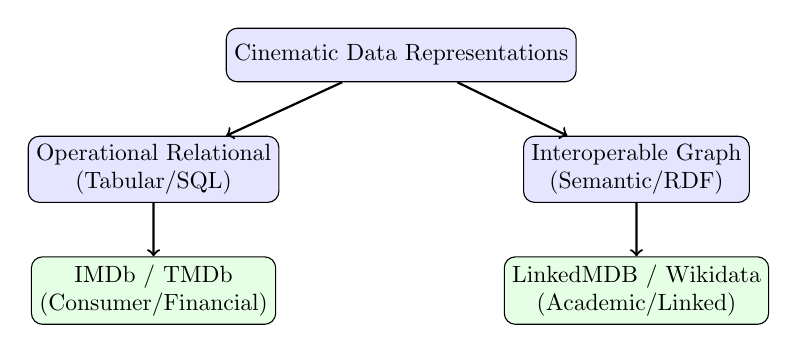
\begin{tikzpicture}[node distance=1.2cm, auto, transform shape, scale=0.85,
    box/.style={draw, rectangle, align=center, fill=blue!10, rounded corners, minimum height=0.8cm, minimum width=2.5cm}]
  
  \node[box] (root) {Cinematic Data Representations};
  
  \node[box, below left=0.8cm and -0.8cm of root] (rel) {Operational Relational\\(Tabular/SQL)};
  \node[box, below right=0.8cm and -0.8cm of root] (graph) {Interoperable Graph\\(Semantic/RDF)};
  
  \node[box, below=0.8cm of rel, fill=green!10] (imdb) {IMDb / TMDb\\(Consumer/Financial)};
  \node[box, below=0.8cm of graph, fill=green!10] (linked) {LinkedMDB / Wikidata\\(Academic/Linked)};

  \draw[->, thick] (root) -- (rel);
  \draw[->, thick] (root) -- (graph);
  \draw[->, thick] (rel) -- (imdb);
  \draw[->, thick] (graph) -- (linked);
\end{tikzpicture}
\caption{Taxonomy of existing cinematic data models.}
\end{figure}

Operational Relational systems (like IMDb and TMDb) are heavily entity-centered, focusing on rapid retrieval of isolated facts (e.g., an actor's filmography). Interoperable Graph systems (like LinkedMDB and Wikidata) are event-centered and semantic, designed to connect data across different web standards, allowing for reasoning over the relationships themselves \cite{semantic}.

\section{Comparative Analysis}
To inform our design, we compared three representative systems: IMDb, TMDb, and LinkedMDB. Table 1 summarizes the key entities, relationships, strengths, and limitations of each.

\begin{table*}[t]
\centering
\caption{Comparison of Existing Cinematic Data Models}
\renewcommand{\arraystretch}{1.2}
\begin{tabularx}{\textwidth}{l l X X X}
\toprule
\textbf{Model} & \textbf{Main Purpose} & \textbf{Key Entities} & \textbf{Strengths} & \textbf{Limitations} \\
\midrule
\textbf{IMDb} & Consumer reference. & Person, Title, Crew. & Massive volume; highly granular role types. & Flat structure; roles are string attributes, not entities. \\
\textbf{TMDb} & Operational analytics. & Movie, Person, Financials. & Strong financial/box office tracking capability. & Relational silos prevent seamless network traversal. \\
\textbf{LinkedMDB} & Semantic interoperability. & Film, Actor, Performance. & High interoperability; explicit semantic relationships. & Outdated; lacks robust financial attributes for commercial use. \\
\bottomrule
\end{tabularx}
\end{table*}

IMDb treats the `Title` as the central entity and associates people via a flat `principals` table. Its strength lies in its massive data volume. However, it simplifies the relationship by treating roles merely as text strings rather than distinct entities, making semantic reasoning difficult \cite{imdb}. TMDb includes robust financial attributes (budget, revenue), which is vital for tracking "blockbusters" and "flops." However, it remains trapped in a relational structure that requires heavy SQL `JOIN` operations to map collaborative networks \cite{tmdb}. 

LinkedMDB represents events more explicitly. By using RDF triples, it distinguishes between the film, the performance, and the actor, allowing for high interoperability \cite{linkedmdb}. However, it lacks the up-to-date financial metrics required by producers.

\section{Positioning and Draft ERD}
Based on our comparative analysis, existing models either lack financial depth (LinkedMDB) or fail to capture relationships as distinct semantic entities (IMDb/TMDb). To address these gaps, we propose the conceptual model illustrated in Figure 2 on the following page. 

Our model introduces several key distinctions intended to support our specific information need and prepare for the eventual transition to a Knowledge Graph. 

First, we elevate `Performance\_Role` to an explicit entity. Rather than a direct many-to-many relationship between `Person` and `Movie`, a `Person` \textit{fills} a `Performance\_Role`, which \textit{belongs to} a `Movie`. This addresses IMDb's limitation, allowing us to attach specific attributes (e.g., character name, billing order) directly to the role. When transitioning to RDF/OWL, this structure translates seamlessly into intermediate graph nodes, preserving semantic richness.

Second, we incorporate financial and critical attributes directly into the `Movie` entity (Budget, Box Office Revenue, Performance Classification) to address LinkedMDB's commercial limitations. This ensures our model can answer queries such as identifying actors who consistently appear in "Blockbuster" classifications alongside specific directors. 

\textbf{Note on Draft Status:} This diagram serves as an initial conceptualization. As we progress toward physical implementation, attribute types, cardinalities, and normalization constraints will be continuously refined \cite{course}.

\bibliographystyle{ACM-Reference-Format}
\begin{thebibliography}{5}
\bibitem{course} CSC501 Course Manual. 2026. \emph{Milestone 2: Background and Related Work}.
\bibitem{semantic} T. Berners-Lee et al. 2001. \emph{The Semantic Web}. Scientific American.
\bibitem{imdb} IMDb. 2026. \emph{Non-Commercial Datasets}.
\bibitem{linkedmdb} O. Hassanzadeh and M. Consens. 2009. \emph{Linked Movie Data Base}.
\bibitem{tmdb} TMDb. 2026. \emph{The Movie Database API}.
\end{thebibliography}

% Force the diagram to a completely new third page
\clearpage

\begin{figure*}[!t]
\centering
\vspace*{1.5cm} % Push the diagram down slightly from the top margin
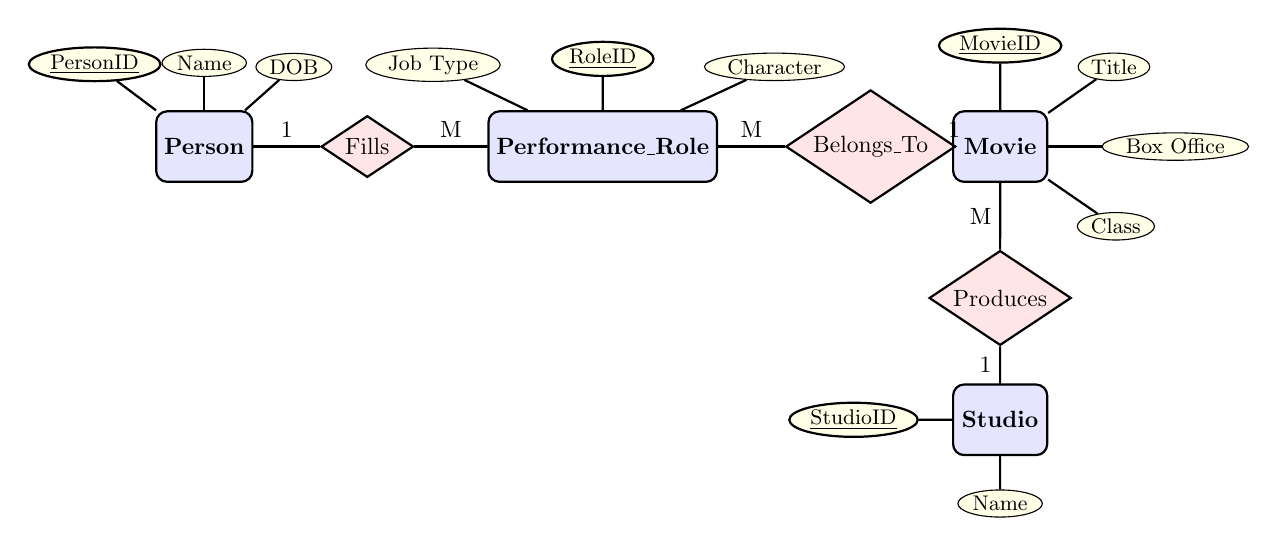
\begin{tikzpicture}[
    auto,
    transform shape, scale=0.85, 
    node distance=2.5cm and 2.5cm,
    entity/.style={rectangle, draw, thick, fill=blue!10, text centered, rounded corners, minimum height=3em, minimum width=4em, font=\bfseries},
    relationship/.style={diamond, draw, thick, fill=red!10, text centered, aspect=1.5, inner sep=2pt},
    attribute/.style={ellipse, draw, fill=yellow!10, text centered, inner sep=1pt, font=\small},
    ident/.style={ellipse, draw, thick, fill=yellow!10, text centered, inner sep=1pt, font=\small},
    line/.style={draw, thick}
]

% Entities
\node[entity] (person) {Person};
\node[entity, right=3.5cm of person] (role) {Performance\_Role};
\node[entity, right=3.5cm of role] (movie) {Movie};
\node[entity, below=3cm of movie] (studio) {Studio};

% Relationships
\node[relationship, right=1cm of person] (fills) {Fills};
\node[relationship, right=1cm of role] (belongs) {Belongs\_To};
\node[relationship, below=1cm of movie] (produces) {Produces};

% Person Attributes
\node[ident, above left=0.5cm and 0.2cm of person] (pid) {\underline{PersonID}};
\node[attribute, above=0.5cm of person] (pname) {Name};
\node[attribute, above right=0.5cm and 0.2cm of person] (pdob) {DOB};
\draw[line] (person) -- (pid);
\draw[line] (person) -- (pname);
\draw[line] (person) -- (pdob);

% Role Attributes
\node[ident, above=0.5cm of role] (rid) {\underline{RoleID}};
\node[attribute, above left=0.5cm and 0.1cm of role] (rtype) {Job Type};
\node[attribute, above right=0.5cm and 0.1cm of role] (char) {Character};
\draw[line] (role) -- (rid);
\draw[line] (role) -- (rtype);
\draw[line] (role) -- (char);

% Movie Attributes - Spaced out wider into a clean semi-circle
\node[ident, above=0.7cm of movie] (mid) {\underline{MovieID}};
\node[attribute, above right=0.5cm and 0.6cm of movie] (title) {Title};
\node[attribute, right=0.8cm of movie] (box) {Box Office};
\node[attribute, below right=0.5cm and 0.6cm of movie] (class) {Class};
\draw[line] (movie) -- (mid);
\draw[line] (movie) -- (title);
\draw[line] (movie) -- (box);
\draw[line] (movie) -- (class);

% Studio Attributes
\node[ident, left=0.5cm of studio] (sid) {\underline{StudioID}};
\node[attribute, below=0.5cm of studio] (sname) {Name};
\draw[line] (studio) -- (sid);
\draw[line] (studio) -- (sname);

% Connections - Traditional Chen's Notation
\draw[line] (person) -- node[above] {1} (fills);
\draw[line] (fills) -- node[above] {M} (role);

\draw[line] (role) -- node[above] {M} (belongs);
\draw[line] (belongs) -- node[above] {1} (movie);

\draw[line] (studio) -- node[left] {1} (produces);
\draw[line] (produces) -- node[left] {M} (movie);

\end{tikzpicture}
\caption{Draft Entity-Relationship Diagram modeling the cinematic domain. `Performance\_Role` explicitly bridges `Person` and `Movie`.}
\end{figure*}

\end{document}